\section{Orthogonalprojektion}
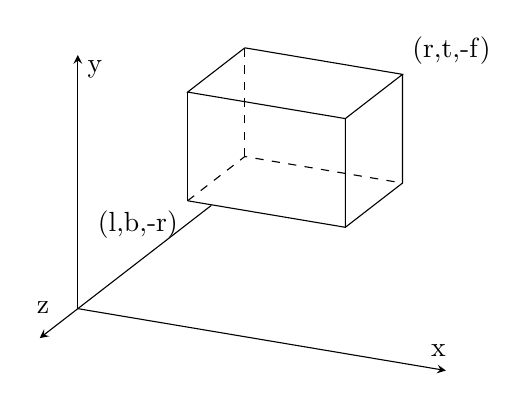
\begin{tikzpicture}
\begin{axis}[axis lines = center, xlabel = x, ylabel=z, zlabel = y, xmax=7,ymax=2,zmax=7, ymin=-7, y post scale=-1, ticks=none ]
\addplot3[draw=none] coordinates {(0,0,0)};
\draw (axis cs:1,-3,2)--(axis cs:4,-3,2)--(axis cs:4,-3,5) -- (axis cs:1,-3,5)--(axis cs:1,-6,5);
\draw[dashed] (axis cs:1,-3,2)--(axis cs:1,-6,2) -- (axis cs:4,-6,2) ;
\draw[dashed] (axis cs:1,-6,2)--(axis cs:1,-6,5);
\draw (axis cs:1,-3,2)--(axis cs:1,-3,5);
\draw (axis cs:1,-6,5)--(axis cs:4,-6,5)--(axis cs:4,-3,5);
\draw (axis cs:4,-3,2)--(axis cs:4,-6,2)--(axis cs:4,-6,5);
\node[anchor=north east] at (axis cs:1,-3,2) {(l,b,-r)};
\node[anchor=south west] at (axis cs:4,-6,5) {(r,t,-f)};
\end{axis}
\end{tikzpicture}
\begin{align*}
x \in [l,r]\\
y \in [b,t]\\
z \in [-f, -n]
\end{align*}
Sichtquader $\rightarrow$ Einheitsquader

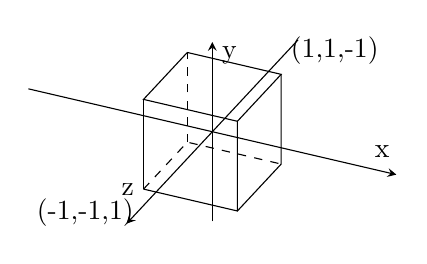
\begin{tikzpicture}
\begin{axis}[axis lines = center, xlabel = x, ylabel=z, zlabel = y, xmax=2,ymax=2,zmax=2, xmin=-2, ymin=-2, zmin=-2, y post scale=-1, axis equal, ticks=none]
\addplot3[draw=none] coordinates {(0,0,0)};
\draw (axis cs:-1,1,-1)--(axis cs:1,1,-1)--(axis cs:1,1,1) -- (axis cs:-1,1,1)--(axis cs:-1,-1,1);
\draw[dashed] (axis cs:-1,1,-1)--(axis cs:-1,-1,-1) -- (axis cs:1,-1,-1) ;
\draw[dashed] (axis cs:-1,-1,-1)--(axis cs:-1,-1,1);
\draw (axis cs:-1,1,-1)--(axis cs:-1,1,1);
\draw (axis cs:-1,-1,1)--(axis cs:1,-1,1)--(axis cs:1,1,1);
\draw (axis cs:1,1,-1)--(axis cs:1,-1,-1)--(axis cs:1,-1,1);
\node[anchor=north east] at (axis cs:-1,1,-1) {(-1,-1,1)};
\node[anchor=south west] at (axis cs:1,-1,1) {(1,1,-1)};
\end{axis}
\end{tikzpicture}
\begin{align*}
x' \in [-1,1]\\
y' \in [-1,1]\\
z' \in [-1, 1]
\end{align*}

\begin{align*}
x' = a\alpha \cdot x + \beta\\
l \mapsto -1, ~ r\mapsto 1
\end{align*}
\begin{align*}
(1)&&-1 = \alpha\cdot l + \beta\\
(2)&& 1 = \alpha\cdot r + \beta\\
\hline
(2) - (1)&& 2 = \alpha\cdot r -\alpha\cdot l \Rightarrow \alpha = \frac{2}{r-l}\\
&&1 = \frac{2\cdot r}{r - l}+\beta\\
&&\beta = 1 - \frac{2r}{r-l} = \frac{r-l-2r}{r-e} = -\frac{r+l}{r-l}
\end{align*}
\[ \underset{\text{NDS}}{\vektor{x'\\y'\\z'\\1}} = \underset{Q}{\underbrace{\vektor{\frac{2}{r-l}&0&0&\frac{r+l}{r-l}\\0&\frac{2}{t-b}&0&\frac{t+b}{t-b}\\0&0&\frac{-2}{f-n}&-\frac{f+n}{f-n}\\0&0&0&1   }}}\cdot\vektor{x\\y\\z\\1} \]
\[  z' = -\frac{2}{f-n}z - \frac{f+n}{f-n}  \]
\[ z=n~~~z* = \frac{2n-(f+n)}{f-n} = \frac{n-f}{f-n} = -1 \]
\[ -n\mapsto -1,~-f\mapsto 1\]
\texttt{Qmatrix4x4.ortho(l,n,b,t,n,f);}
\section{Perspektivische Projektion}
%Bild 3
\begin{tikzpicture}[scale=1.2]
\begin{axis}[axis lines = center, xlabel = z, ylabel=y, xmin = -5.5, ymin=-1.2, ymax=1.2, xmax=1, ticks=none]
%\addplot[draw=none] coordinates {(0,0)};
\draw[draw=red, fill=none, double distance=0.5] (-1,0.2)--(-5,1) -- (-5,-1)--(-1,-0.2)--(-1,0.2);
\draw (0,0)--(-5,1) -- (-5,-1) node [pos=.6, below] {-f$~~~~$}--(0,0);
\draw (-1,-1)--(-1,1);
\draw[very thick, -{Circle[length=3pt]}] (-1,0)--(-1,0.2);
\draw[double distance = 4, -{Triangle[open, length=8, width=8]}] (-2,0)--(-2,0.4);
\draw[double distance = 4, -{Triangle[open, length=8, width=8]}] (-4,0)--(-4,0.8);
\draw[<->] (-1,-0.2)--(0,-0.2) node [pos=.5, below, sloped] {n};
\node[rotate=180,pin=sichtbar, anchor=north] at(axis cs:-2.5, -0.4) {};
\node[anchor=south] at (axis cs:-4,0.8) {(y,z)};
\node[anchor=south west] at (axis cs:-1,0.2) {(y',-n)};
%\node[anchor=north east] at (axis cs:-1,1,-1) {(-1,-1,1)};
%\node[anchor=south west] at (axis cs:1,-1,1) {(1,1,-1)};
\end{axis}
\end{tikzpicture}
\[ \frac{y'}{-n} = \frac{y}{z} \]
\[ y' = - \frac{n\cdot y}{z} \]
Sichtpyramide $\rightarrow$ Einheitswürfel
%Bild 4
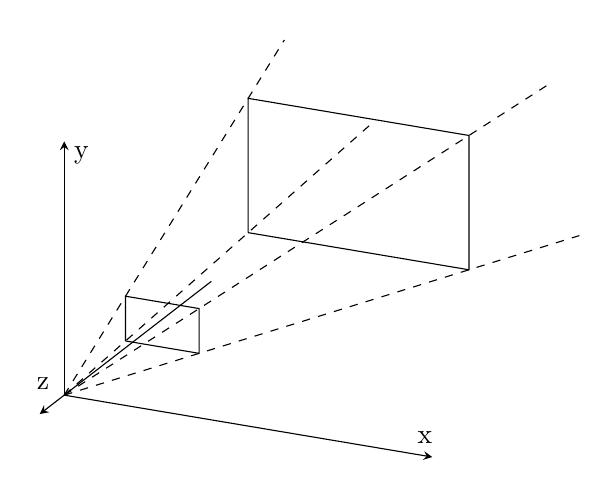
\begin{tikzpicture}
\begin{axis}[axis lines = center, xlabel = x, ylabel=z, zlabel = y, xmax=15,ymax=2,zmax=17, ymin=-12, y post scale=-1, ticks=none ]
\addplot3[draw=none] coordinates {(0,0,0)};
\draw (1,-3,2)--(4,-3,2)--(4,-3,5) -- (1,-3,5)--(1,-3,2);
\draw[dashed] (0,0,0)--(1,-3,2)--(5,-15,10);
\draw[dashed] (0,0,0)--(4,-3,2)--(20,-15,10);
\draw[dashed] (0,0,0)--(4,-3,5)--(20,-15,25);
\draw[dashed] (0,0,0)--(1,-3,5)--(5,-15,25);

\draw (3,-9,6)--(12,-9,6)--(12,-9,15)--(3,-9,15)--(3,-9,6);

\end{axis}
\end{tikzpicture}
\begin{align*}
y'&=-\frac{n\cdot y}{z}\\[-1.25em]
\rotatebox{-90}{$\in$}~& \\
[b,t]&\mapsto[-1,1]\\
&y'' = \alpha\cdot y' + \beta\\
&y'' = \frac{2}{t\cdot b}\cdot y' - \frac{t+b}{t-b}\\
&\boxed{y'' = \frac{-2n}{t-b}\cdot \frac{y}{z} - \frac{t+b}{t-b} }
\end{align*}

\[ \underset{\text{homogene Koord.}}{\vektor{x\\y\\z\\w}}\overset{\text{Dehomogen-}}{\underset{\text{isierung}}{\longrightarrow}}\underset{\text{Kartesiche koord.}}{\vektor{\frac{x}{w}\\ \frac{y}{w}\\ \frac{z}{w}}} \]
\[ \vektor{x''\\ y''\\ z''\\ w''} = \vektor{\frac{2n}{r-l} & 0 & \frac{r+l}{r-l} & 0 \\0 & \frac{2n}{t-b} & -\frac{t+b}{t-b} & 0 \\ 0& 0&\alpha &\beta \\ 0&0&-1&0   } \cdot \vektor{x\\y\\z\\1} \]
\[ y'' = \frac{2n}{t-b}\cdot y + \frac{t + b}{t- b}\cdot z \]
\[ w'' = -z \]
\[ \frac{y''}{w''} = \frac{2n}{t-b}\frac{y}{(-z)} + \frac{t+b}{t-b}\frac{z}{(-z)} \]

\[ z''' = \frac{z''}{w''} = \frac{\alpha\cdot z + \beta}{- z} = -\alpha-\frac{\beta}{z} \]
\[ -n\mapsto -1,~-f \mapsto 15 \]

\begin{align*}
 -\alpha- \frac{\beta}{-n} = -1& \\ 
 -\alpha-\frac{\beta}{-f} = 1 & \\
 -\alpha + \frac{\beta}{n} = -1 &(1)\\
 -\alpha+\frac{\beta}{f} = 1&(2)\\
\hline\\
\frac{\beta}{f} - \frac{\beta}{n} = 2 &(2)-(1)\\
\beta\left( \frac{1}{f}-\frac{1}{n} \right) = 2& \\
\beta\left(\frac{n-f}{fn}\right)& \\
\beta = \frac{-2nf}{f-n}& \\
\alpha = \frac{\beta}{f} - 1 = -\frac{2n-(f-n)}{f-n} = \frac{f+n}{f-n}&
\end{align*}
\[ p' = \underset{\text{die Welt-x-Achse}}{\underset{\text{Drehung um}}{\underset{\uparrow}{\underset{\footnotesize\textcircled{2}}{R_{\vartheta, x}}}}} \cdot \underset{\text{die Welt-y-Achse}}{\underset{\text{Drehung um}}{\underset{\uparrow}{\underset{\footnotesize\textcircled{1}}{R_{\varphi, y}}}}}\cdot p \]
%Bild mit 3d koord sys und dre pfeilen um y und x achse 
